\let\negmedspace\undefined
\let\negthickspace\undefined
\documentclass[journal]{IEEEtran}
\usepackage[a5paper, margin=10mm, onecolumn]{geometry}
\usepackage{lmodern} % Ensure lmodern is loaded for pdflatex
\usepackage{tfrupee} % Include tfrupee package

\setlength{\headheight}{1cm} % Set the height of the header box
\setlength{\headsep}{0mm}     % Set the distance between the header box and the top of the text

\usepackage{gvv-book}
\usepackage{gvv}
\usepackage{cite}
\usepackage{amsmath,amssymb,amsfonts,amsthm}
\usepackage{algorithmic}
\usepackage{graphicx}
\usepackage{textcomp}
\usepackage{xcolor}
\usepackage{txfonts}
\usepackage{listings}
\usepackage{enumitem}
\usepackage{mathtools}
\usepackage{gensymb}
\usepackage{comment}
\usepackage[breaklinks=true]{hyperref}
\usepackage{tkz-euclide} 
\usepackage{listings}
\usepackage{gvv}                                        
\def\inputGnumericTable{}                                 
\usepackage[latin1]{inputenc}                                
\usepackage{color}                                            
\usepackage{array}                                            
\usepackage{longtable}                                       
\usepackage{calc}                                             
\usepackage{multirow}                                         
\usepackage{hhline}                                           
\usepackage{ifthen}                                           
\usepackage{lscape}
\begin{document}

\bibliographystyle{IEEEtran}
\vspace{3cm}

\title{9-9.2-5}
\author{EE24BTECH11036 - Krishna Patil}
% \maketitle
% \newpage
% \bigskip
{\let\newpage\relax\maketitle}
Question: \\
 Find the area of the region bounded by the ellipse $ \frac{x^2}{4} + \frac{y^2}{9} = 1 $ . 
 \\ \\
\solution \\ \\
Equation of a conic in matrix form is : \\
\begin{align}
    x^\top V x + 2u^\top {x} + f = 0
\end{align} \\ 
For given ellipse, \\
\begin{align}
    V&= \myvec{1 & 0 \\ 0 & \frac{4}{9}} \\
    u&= \myvec{0 \\ 0} \\
    f&=-4 
\end{align}
$ \therefore $ Area of the ellipse is  
\begin{align}
    A &= 4 \int_{0}^{2} 3 \sqrt{1 - \frac{x^2}{4}} \, dx\ \\
    A &= 6\pi
\end{align}
\begin{table}[h!]    	
    \centering
    % Assuming the table.tex file exists
    \begin{tabular}[12pt]{|c|c|c|}
    \hline
    Parameter & Description & Values\\ 
    \hline
    $V$ & $\myvec{ 1 & 0 \\ 0 & 1-e^{2} }$ & $\myvec{1 & 0 \\ 0 & \frac{4}{9} }$ \\
    \hline
    $u$ & - & $\myvec{0 \\ 0}$ \\
    \hline
    $f$ & $b^2(e^2 -1)$ & -4 \\
    \hline
    $A$ & Area under Curve & $6\pi$ \\
    \hline
    \end{tabular}
 
    \caption{Parameters Used}
    \label{tab:1-1.9-6}
\end{table}
\begin{figure}[ht]
    \centering
    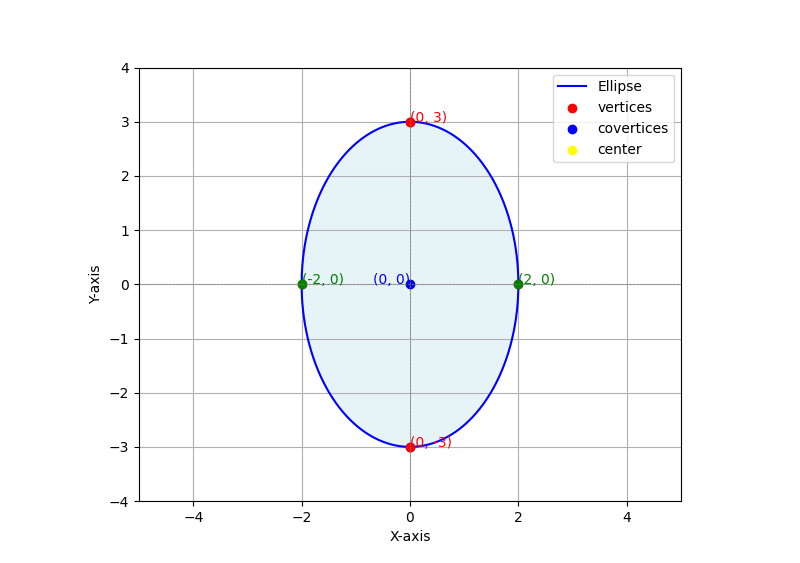
\includegraphics[width = \columnwidth]{figs/Figure_1.png}
    \caption{Plot of ellipse}
    \label{fig:stemplot}
\end{figure}

\end{document}

